\documentclass[a4paper]{article}

%use the english line for english reports
%usepackage[english]{babel}
\usepackage[portuguese]{babel}
\usepackage[utf8]{inputenc}
\usepackage{indentfirst}
\usepackage{graphicx}
\usepackage{subfig}
\usepackage{verbatim}
\usepackage{listings} 
\usepackage{multicol}

\begin{document}

\setlength{\textwidth}{16cm}
\setlength{\textheight}{22cm}

\title{\Huge\textbf{MOD X}\linebreak\linebreak\linebreak
\Large\textbf{Relatório Intercalar}\linebreak\linebreak
\linebreak\linebreak

\includegraphics[scale=0.1]{./images/feup-logo.png}\linebreak\linebreak
\linebreak\linebreak
\Large{Mestrado Integrado em Engenharia Informática e Computação} \linebreak\linebreak
\Large{Programação em Lógica}\linebreak
}

\author{\textbf{Grupo Mod X\_3:}\\
António Manuel Vieira Ramadas - 201303568 \\
Rui Miguel Teixeira Vilares - 201207046 \\
\linebreak\linebreak \\
 \\ Faculdade de Engenharia da Universidade do Porto \\ Rua Roberto Frias, s\/n, 4200-465 Porto, Portugal \linebreak\linebreak\linebreak
\linebreak\linebreak\vspace{1cm}}

\maketitle
\thispagestyle{empty}

%************************************************************************************************
%************************************************************************************************

\newpage

%Todas as figuras devem ser referidas no texto. %\ref{fig:codigoFigura}
%
%%Exemplo de código para inserção de figuras
%%\begin{figure}[h!]
%%\begin{center}
%%escolher entre uma das seguintes três linhas:
%%\includegraphics[height=20cm,width=15cm]{path relativo da imagem}
%%\includegraphics[scale=0.5]{path relativo da imagem}
%%\includegraphics{path relativo da imagem}
%%\caption{legenda da figura}
%%\label{fig:codigoFigura}
%%\end{center}
%%\end{figure}
%
%
%\textit{Para escrever em itálico}
%\textbf{Para escrever em negrito}
%Para escrever em letra normal
%``Para escrever texto entre aspas''
%
%Para fazer parágrafo, deixar uma linha em branco.
%
%Como fazer bullet points:
%\begin{itemize}
	%\item Item1
	%\item Item2
%\end{itemize}
%
%Como enumerar itens:
%\begin{enumerate}
	%\item Item 1
	%\item Item 2
%\end{enumerate}
%
%\begin{quote}``Isto é uma citação''\end{quote}


%%%%%%%%%%%%%%%%%%%%%%%%%%
\section{O Jogo MOD X\newline}

\subsection{Contextualização}
O MOD X é um jogo de tabuleiro, criado em 2015, recomendado para jogadores com mais de 15 anos de idade.
É um jogo de estratégia, divertido e fácil de aprender.
Cada partida reúne 2 a 4 jogadores e tem a duração prevista de 20 a 30 minutos. 

\subsection{Componentes do jogo}
\begin{itemize}
	\item 1 Tabuleiro 8x8;
	\item 56 peças de jogo em formato X (14 em cada cor);
	\item 72 marcadores de pontuação (18 em cada cor);
	\item 5 peças \textit{Joker} em formato X (brancas);
\end{itemize}

\begin{figure}[h!]
	\begin{center}
		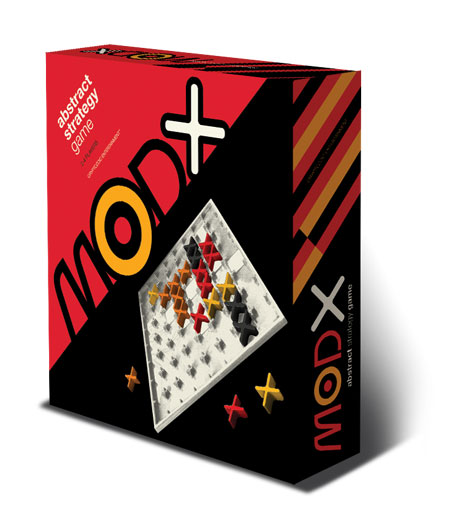
\includegraphics[scale=0.3]{./images/modx_box.jpg}
		\caption{Caixa do MOD X}
		\label{fig:1}
	\end{center}
\end{figure}

\subsection{Objetivo do jogo}

O objetivo deste jogo é criar padrões com peças coloridas (vermelho, preto, amarelo ou laranja).
Pretende-se assim, formar o maior número de padrões possível, de forma a conseguir a melhor pontuação.
O vencedor é o jogador com mais pontos.
Evidentemente, é também suposto bloquear os adversários de modo que não consigam construir esses padrões\footnote{https://boardgamegeek.com/boardgame/131387/mod-x}.  

\subsection{Regras}

\begin{itemize}
	\item Define-se a ordem dos jogadores, cada um escolhe a cor das suas peças e define-se o limite de pontos\footnote{https://www.cryptozoic.com/games/mod-x};
	\item Cada jogador inicia o jogo com 14 peças e 18 marcadores;
	\item Os \textit{Jokers} são dispostos inicialmente de forma aleatória no tabuleiro; 
	\item No seu turno, cada jogador coloca uma peça no tabuleiro, em qualquer posição livre;
	\item Os padrões utilizados para ganhar pontos são o ''X'', o ''+'' e o ''cinco em linha'';
	
	\begin{figure}[h!]
		\begin{center}
			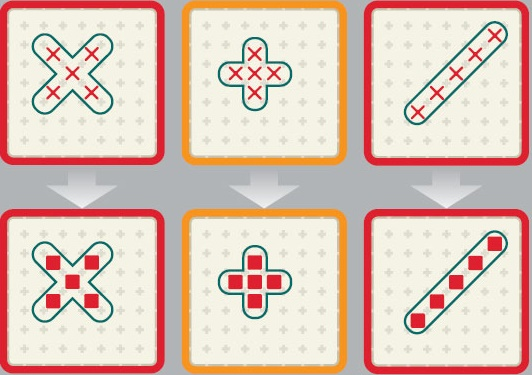
\includegraphics[scale=0.4]{./images/modx_score.jpg}
			\caption{Padrões usados}
			\label{fig:2}
		\end{center}
	\end{figure}
	
	\item O jogador pode usar os \textit{Jokers} para formar padrões, como se das suas próprias peças se tratassem;
	\item Quando um padrão é formado, retiram-se as peças de jogo e introduzem-se marcadores nessas posições. As peças de jogo podem agora voltar a ser utilizadas e as casas com marcadores também;
	\item Cada marcador colocado corresponde a um ponto;
	\item Caso tenha sido usado um \textit{Joker} para formar um padrão, nessa posição não é introduzido um marcador. O \textit{Joker} é agora colocado numa posição ao critério do jogador. Atenção, o \textit{Joker} não pode ser usado para formar um novo padrão de imediato; 
	
	\begin{figure}[!h]
		\centering
		\subfloat[Peças]{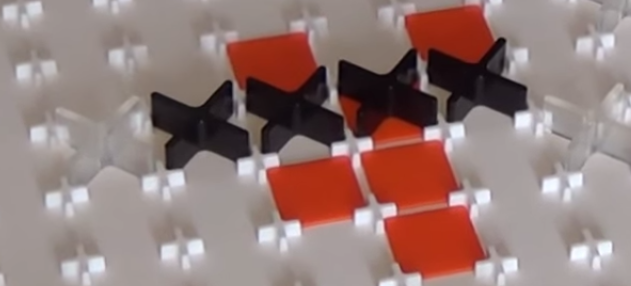
\includegraphics[width=0.3\textwidth]{./images/padroesPretos.png}\label{fig:3}}
		\hfill
		\subfloat[Marcadores]{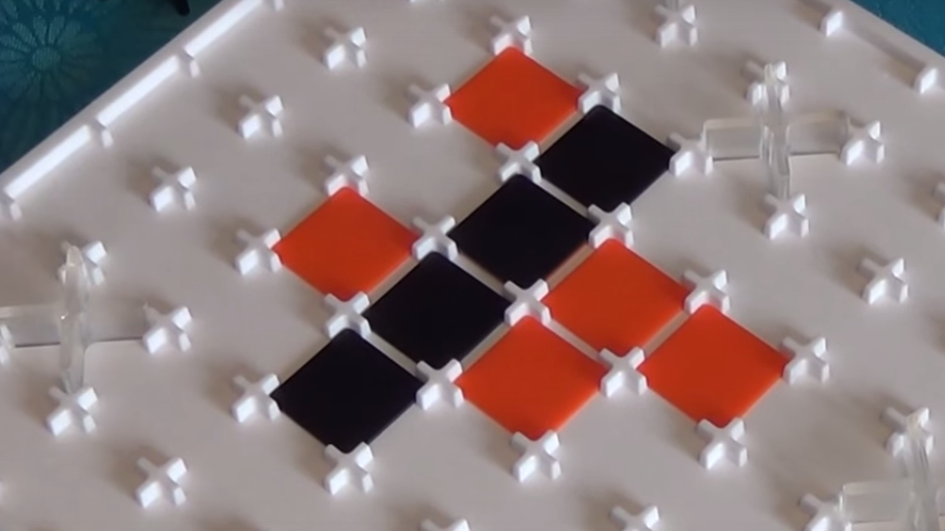
\includegraphics[width=0.3\textwidth]{./images/padroesPretosMarcadores.png}\label{fig:4}}
		\caption{Substituição das peças por marcadores}
	\end{figure}
	
	\item O primeiro jogador a atingir o número de pontos, determinado inicialmente, é o vencedor;
	\item O jogo pode também acabar quando um jogador já não dispõe de peças ou marcadores. Nesse caso, ganha o jogador com mais pontos até ao momento\footnote{https://youtu.be/pto-7O618rI};
	

	
\end{itemize}
%%Cada jogador inicia o jogo com 14 peças e 18 marcadores.
%%Inicialmente, define-se a ordem dos jogadores e escolha das peças por parte dos jogadores.  
%%No seu turno, um jogador coloca uma peça no tabuleiro, com o objetivo de criar padrões específicos, que se traduzem em pontos.
%%Os padrões utilizados para ganhar pontos são o ''X'', o ''+'' e o ''cinco em linha''.

%%Existem umas peças de cor branca, dispostas inicialmente de forma aleatória, chamadas Jokers. O jogador pode usar essas peças para formar padrões, como se tratassem das suas próprias peças.

%%É suposto bloquear os adversários de modo que não consigam construir esses padrões\footnote{https://www.cryptozoic.com/games/mod-x}.

%%No final, o primeiro jogador a atingir um certo número de pontos, determinado inicialmente pelo número de jogadores, é o vencedor.
%%O jogo pode também terminar quando um jogador terminar com as suas peças ou marcadores.
%%Nesse caso, o jogo termina imediatamente e ganha o jogador com mais pontos até ao momento.


%%%%%%%%%%%%%%%%%%%%%%%%%%


\begin{multicols}{2}
	[\section{Representação do Estado do Jogo\newline}]
Na representação exterior, ou seja, quando o tabuleiro é visualizado pelo utilizador, usamos as seguintes propriedades:
\begin{itemize}
	\item Peças de jogo:
		\begin{itemize}
			\item espaço em branco = livre (vazio)
			\item 0 = \textit{Joker} (transparente)
			\item 1 = jogador 1
			\item 2	= jogador 2
		\end{itemize}
	\item Marcadores:
		\begin{itemize}
			\item espaço em branco = vazio
			\item * = marcador do jogador 1
			\item : = marcador do jogador 2
		\end{itemize}
\end{itemize}

\columnbreak

Na representação interna, ou seja, nos dados armazenados pelo computador, usamos a seguinte sintaxe:
\begin{itemize}
	\item Peças de jogo:
	\begin{itemize}
		\item -1 = livre (vazio)
		\item 0 = \textit{joker} (transparente)
		\item 1 = jogador 1
		\item 2 = jogador 2
	\end{itemize}
	\item Marcadores:
	\begin{itemize}
		\item -1 = vazio
		\item 11 = base do jogador 1
		\item 22 = base do jogador 2
	\end{itemize}
\end{itemize}

\end{multicols}

\subsection{Representação de um estado inicial do tabuleiro}

%%printBoard(
\begin{small}
\begin{lstlisting}
[[-1,-1],[-1,-1],[-1,-1],[-1,-1],[-1,-1],[-1,-1],[-1,-1],[-1,-1],
[-1,-1],[0,-1],[-1,-1],[-1,-1],[-1,-1],[-1,-1],[-1,-1],[-1,-1],
[-1,-1],[-1,-1],[-1,-1],[-1,-1],[-1,-1],[-1,-1],[-1,-1],[-1,-1],
[0,-1],[-1,-1],[-1,-1],[-1,-1],[-1,-1],[0,-1],[-1,-1],[-1,-1],
[-1,-1],[-1,-1],[-1,-1],[-1,-1],[-1,-1],[-1,-1],[0,-1],[-1,-1],
[-1,-1],[-1,-1],[-1,-1],[-1,-1],[-1,-1],[-1,-1],[-1,-1],[-1,-1],
[-1,-1],[-1,-1],[0,-1],[-1,-1],[-1,-1],[-1,-1],[-1,-1],[-1,-1],
[-1,-1],[-1,-1],[-1,-1],[-1,-1],[-1,-1],[-1,-1],[-1,-1],[-1,-1]]
\end{lstlisting}
\end{small}
%%).

\begin{figure}[h!]
	\begin{center}
		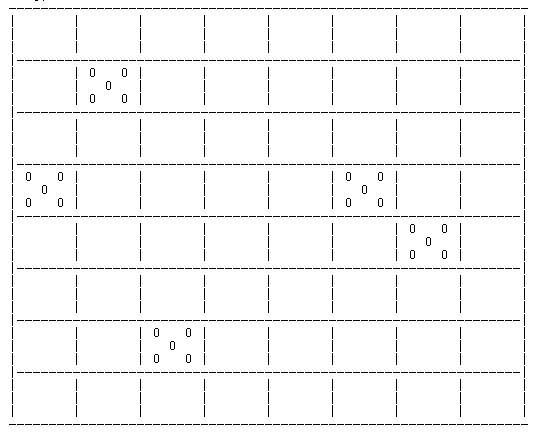
\includegraphics[scale=0.4]{./images/inicial.png}
		\caption{Exemplo de um estado inicial}
		\label{fig:5}
	\end{center}
\end{figure}

\vspace{15 mm}

\subsection{Representação de um estado intermédio do tabuleiro}

\begin{small}
\begin{lstlisting}
[[-1,-1],[2,-1],[-1,-1],[-1,-1],[-1,-1],[-1,-1],[-1,11],[-1,-1],
[-1,-1],[0,-1],[-1,-1],[-1,-1],[-1,-1],[-1,11],[-1,11],[-1,11],
[-1,-1],[-1,-1],[-1,-1],[-1,-1],[-1,-1],[-1,-1],[-1,11],[-1,-1],
[-1,-1],[-1,22],[-1,22],[-1,22],[-1,22],[0,-1],[-1,-1],[1,-1],
[0,-1],[-1,-1],[-1,-1],[-1,-1],[-1,-1],[-1,-1],[0,-1],[-1,-1],
[-1,-1],[-1,-1],[-1,-1],[-1,-1],[-1,-1],[1,-1],[-1,-1],[1,-1],
[2,-1],[2,-1],[0,-1],[2,-1],[1,-1],[-1,-1],[-1,-1],[-1,-1],
[-1,-1],[-1,-1],[-1,-1],[-1,-1],[-1,-1],[-1,-1],[-1,-1],[0,-1]]
\end{lstlisting}
\end{small}

\begin{figure}[h!]
	\begin{center}
		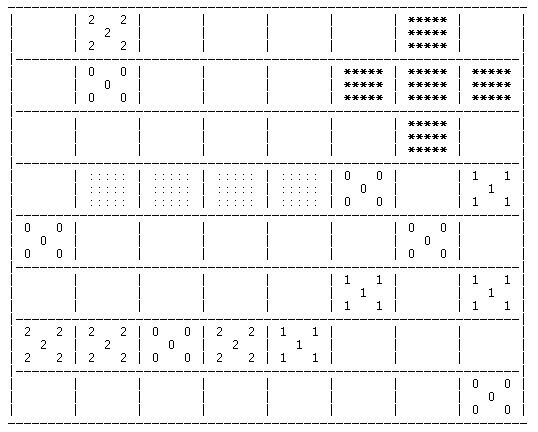
\includegraphics[scale=0.4]{./images/intermedio.png}
		\caption{Exemplo de um estado intermédio}
		\label{fig:6}
	\end{center}
\end{figure}

\subsection{Representação de um estado final do tabuleiro}

\begin{small}
\begin{lstlisting}
[[0,-1],[2,-1],[-1,-1],[-1,-1],[-1,-1],[-1,-1],[-1,11],[0,-1],
[-1,-1],[0,-1],[-1,-1],[-1,-1],[2,-1],[2,11],[-1,11],[-1,11],
[-1,-1],[-1,-1],[-1,-1],[-1,-1],[-1,-1],[-1,-1],[-1,11],[-1,-1],
[-1,-1],[-1,22],[1,22],[-1,22],[-1,22],[-1,-1],[-1,-1],[-1,11],
[0,-1],[-1,-1],[1,-1],[-1,-1],[-1,-1],[-1,-1],[-1,-1],[-1,-1],
[-1,-1],[-1,-1],[-1,22],[0,-1],[-1,-1],[-1,11],[-1,-1],[-1,11],
[2,-1],[-1,22],[-1,-1],[-1,22],[1,-1],[-1,-1],[-1,-1],[-1,-1],
[-1,-1],[-1,-1],[-1,22],[-1,-1],[-1,-1],[-1,-1],[-1,-1],[0,-1]]
\end{lstlisting}
\end{small}

\begin{figure}[h!]
	\begin{center}
		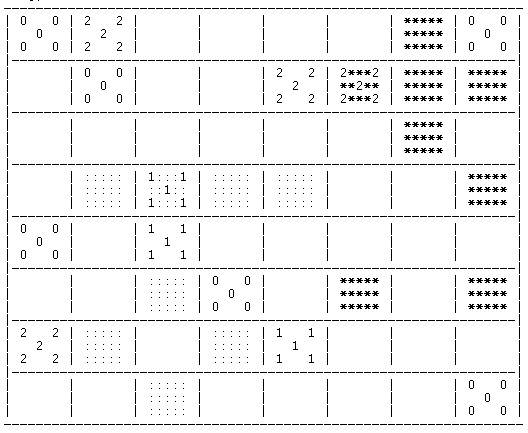
\includegraphics[scale=0.4]{./images/final.png}
		\caption{Exemplo de um estado final}
		\label{fig:7}
	\end{center}
\end{figure}

%%%%%%%%%%%%%%%%%%%%%%%%%%
\section{Visualização do Tabuleiro\newline}

A visualização do tabuleiro em modo de texto é feita através da composição
de caracteres ASCII, como visto anteriormente. Para este efeito, foram desenvolvidos um conjunto de predicados. 

O predicado principal é:
\begin{itemize}
	\item \textbf{printBoard(Board)}: recebe uma lista descritiva das peças que constituem o tabuleiro e imprime-o;
\end{itemize}

Os predicados auxiliares são:
\begin{itemize}

	\item \textbf{printBoardAux(Board, CurrentNumberVertical)}: chamada auxiliar de \textit{printBoard} que desenha \textit{(Board.length mod 8)} vezes;	
	\item \textbf{printHorizontalLine(NumberOfDashes)}: imprime o número de travessões horizontais pretendido;
	\item \textbf{printBlock(Line)}: imprime todos os blocos de uma determinada linha (horizontal);
	\begin{itemize}
		\item \textbf{printLine1(' ', Tile)}: imprime a primeira linha do bloco;
		\item \textbf{print1(' ', Tile)}: predicado auxiliar de \textit{printLine1}, usada para a chamada recursiva;
		\item \textbf{printLine2(' ', Tile)}: imprime a segunda linha do bloco;
		\item \textbf{print2(' ', Tile)}: predicado auxiliar de \textit{printLine2}, usada para a chamada recursiva;
		\item \textbf{printLine3(' ', Tile)}: imprime a terceira linha do bloco;
		\item \textbf{print3(' ', Tile)}: predicado auxiliar de \textit{printLine3}, usada para a chamada recursiva;
		\item \textbf{toPrintMiddle(N)}: verifica se 
		\begin{math}
			N>0 \wedge N<8;
		\end{math}
		\item \textbf{printBeginning(\_)}: imprime o travessão vertical da primeira linha do bloco;
		\item \textbf{printMiddle(\_)}: imprime o travessão vertical da segunda linha do bloco;
		\item \textbf{printEnd(\_)}: imprime o travessão vertical da terceira linha do bloco;
	\end{itemize}
	\item \textbf{convertCode([Cross\textbar Tile], X, Y)}: traduz o átomo em peça de jogo;
	\begin{itemize}
		\item \textbf{convertCodeAux(Cross, [Tile\textbar \_], X, Y)}: predicado auxiliar de \textit{convertCode};
		\item \textbf{translateCodeToChar(X, Y)}: traduz o código X para o código Y;
	\end{itemize}
	\item \textbf{printInfo(\_)}: apresenta informação à cerca da representação do jogo;
	
	\begin{figure}[h!]
		\begin{center}
			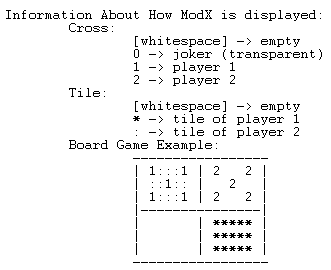
\includegraphics[scale=0.7]{./images/info.png}
			\caption{Informação geral apresentada}
			\label{fig:8}
		\end{center}
	\end{figure}

\end{itemize}
\vspace{10 mm}

%%%%%%%%%%%%%%%%%%%%%%%%%%
\section{Movimentos\newline}

\begin{center}
\textbf{placeJoker(Board, Player, TileNumber).}
\end{center}
Função usada para colocar o \textit{Joker} numa posição específica. Falha se for escolhida numa posição incompatível.\newline

\begin{center}
\textbf{validMoves(Board, Player, ListOfMoves).}
\end{center}
Devolve as jogadas possíveis em \textit{ListOfMoves}.\newline

\begin{center}
\textbf{move(Board, Player, TileNumber, NewBoard).}
\end{center}
Coloca uma nova peça de jogo no tabuleiro. Falha se a peça não poder ser adicionada naquela posição.\newline

\begin{center}
\textbf{value(Board, Player, TileNumber, Value).}
\end{center}
Avalia a jogada e devolve o seu valor em \textit{Value}.\newline

\begin{center}
\textbf{gameOver(Board, Winner).}
\end{center}
Caso o jogo tenha acabado, devolve o vencedor em \textit{Winner}.\newline

\begin{center}
\textbf{choose\_Move(Board, Level, Move).}
\end{center}
Função em que consoante os diferentes níveis de dificuldade (\textit{Level}) devolve jogadas possíveis.\newline

\begin{center}
\textbf{putTiles(Board, Player, NewBoard).}
\end{center}
Substitui as peças de jogo pelos marcadores do \textit{Player}.


\end{document}
